\documentclass[10pt]{beamer}
\usetheme[
%%% options passed to the outer theme
%    progressstyle=fixedCircCnt,   %either fixedCircCnt, movCircCnt, or corner
%    rotationcw,          % change the rotation direction from counter-clockwise to clockwise
%    shownavsym          % show the navigation symbols
  ]{AAUsimple}
  
% If you want to change the colors of the various elements in the theme, edit and uncomment the following lines
% Change the bar and sidebar colors:
%\setbeamercolor{AAUsimple}{fg=red!20,bg=red}
%\setbeamercolor{sidebar}{bg=red!20}
% Change the color of the structural elements:
%\setbeamercolor{structure}{fg=red}
% Change the frame title text color:
%\setbeamercolor{frametitle}{fg=blue}
% Change the normal text color background:
%\setbeamercolor{normal text}{fg=black,bg=gray!10}
% ... and you can of course change a lot more - see the beamer user manual.

\usepackage[utf8]{inputenc}
\usepackage[english]{babel}
\usepackage[T1]{fontenc}
\usepackage{mathenv}
\usepackage{empheq}
\usepackage{subfigure}
\usepackage{multimedia}
\usepackage{pgf,tikz}
\usetikzlibrary{arrows}
%\usepackage[pdftex]{hyperref}

\usepackage{mathtools}
\mathtoolsset{showonlyrefs=true}

\usepackage{multicol}
\usepackage{empheq}
\usepackage{textpos}
\usepackage{graphics}
% Or whatever. Note that the encoding and the font should match. If T1
% does not look nice, try deleting the line with the fontenc.
\usepackage{helvet}

% colored hyperlinks
\newcommand{\chref}[2]{%
  \href{#1}{{\usebeamercolor[bg]{AAUsimple}#2}}%
}
\newcommand{\scaption}[1]{\caption{\tiny{#1}}}



\title{Bernstein-Bézier Polynomial Basis Presentation}

%\subtitle{v.\ 1.2.1}  % could also be a conference name

\date{\today}

\author{
  Pierre Jacquet\\
  \href{mailto:pierre.jacquet@inria.fr}{{\tt pierre.jacquet@inria.fr}}
}

% - Give the names in the same order as they appear in the paper.
% - Use the \inst{?} command only if the authors have different
%   affiliation. See the beamer manual for an example

\institute[
%  {\includegraphics[scale=0.2]{aau_segl}}\\ %insert a company, department or university logo
  First year PhD Student\\
  Inria - Magique 3D - DIP\\
  Pau, FRANCE
] % optional - is placed in the bottom of the sidebar on every slide
{% is placed on the bottom of the title page
   First year PhD Student\\
   Inria - Magique 3D - DIP\\
  Pau, FRANCE
  %there must be an empty line above this line - otherwise some unwanted space is added between the university and the country (I do not know why;( )
}

% specify a logo on the titlepage (you can specify additional logos an include them in 
% institute command below
\pgfdeclareimage[height=2cm]{titlepagelogo}{AAUgraphics/bandeau.png} % placed on the title page
%\pgfdeclareimage[height=1.5cm]{titlepagelogo2}{AAUgraphics/aau_logo_new} % placed on the title page
\titlegraphic{% is placed on the bottom of the title page
  \pgfuseimage{titlepagelogo}
%  \hspace{1cm}\pgfuseimage{titlepagelogo2}
}

\begin{document}
% the titlepage
{\aauwavesbg%
\begin{frame}[plain,noframenumbering] % the plain option removes the header from the title page
  \titlepage
\end{frame}}
%%%%%%%%%%%%%%%%

% TOC
\begin{frame}{Outline}{}
\tableofcontents
\end{frame}
%%%%%%%%%%%%%%%%
\section{Bézier Curves}
\subsection{Historical Aspect}
\begin{frame}{Bézier Curves}{Historical Aspect}

  \vspace{-1.5cm}
  \begin{figure}[H]
    \begin{minipage}[top]{0.30\linewidth}
      %\vspace{-2cm}
      \centering
      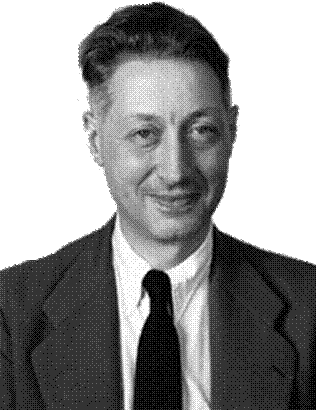
\includegraphics[scale=0.2]{pierre.png}
      \textbf{Pierre Bézier \footnotemark[1]}
    \end{minipage}
    \begin{minipage}[top]{0.65\linewidth}


      %\vspace{-2cm}
      \hspace{2cm}
      \textbf{Dates:} \hspace{0.94cm} 1910-1999


      \hspace{2cm}
      \textbf{Nationality:} \hspace{0.09cm} French
      
      \hspace{2cm}
      \textbf{Institution:}
      
      \hspace{3cm}
      \vspace{-0.95cm}
      \begin{itemize}
        \item[] \hspace{3.54cm}  Arts et Métiers
        \item[]   \hspace{3.54cm} Renault
      \end{itemize}
      \hspace{2cm}
      \textbf{Describes the Curves in 1962}

      
    \end{minipage}
  \end{figure}

  \uncover<2->{
  %\vspace{-1.5cm}
  \begin{figure}[H]
  \begin{minipage}[top]{0.50\linewidth}

      %\vspace{-1cm}
      \hspace{-2cm}
      \textbf{Dates:} \hspace{0.94cm} 1930 - ------
      

      \hspace{-2cm}
      \textbf{Nationality:} \hspace{0.09cm} French


      \hspace{-2cm}
      \textbf{Institution:}
      
      \hspace{-3cm}
      \vspace{-0.95cm}
      \begin{itemize}
        \item[] \hspace{-.46cm}  Ecole Normale Supérieure
        \item[]   \hspace{-0.46cm} Citroën
      \end{itemize}
            \hspace{-2cm}
       \textbf{Describes the Curves in 1958}
      
    \end{minipage}

  \hspace{6.5cm}
    \begin{minipage}[top]{0.30\linewidth}
      \vspace{-3cm}
      \hspace{10cm}
      \centering
      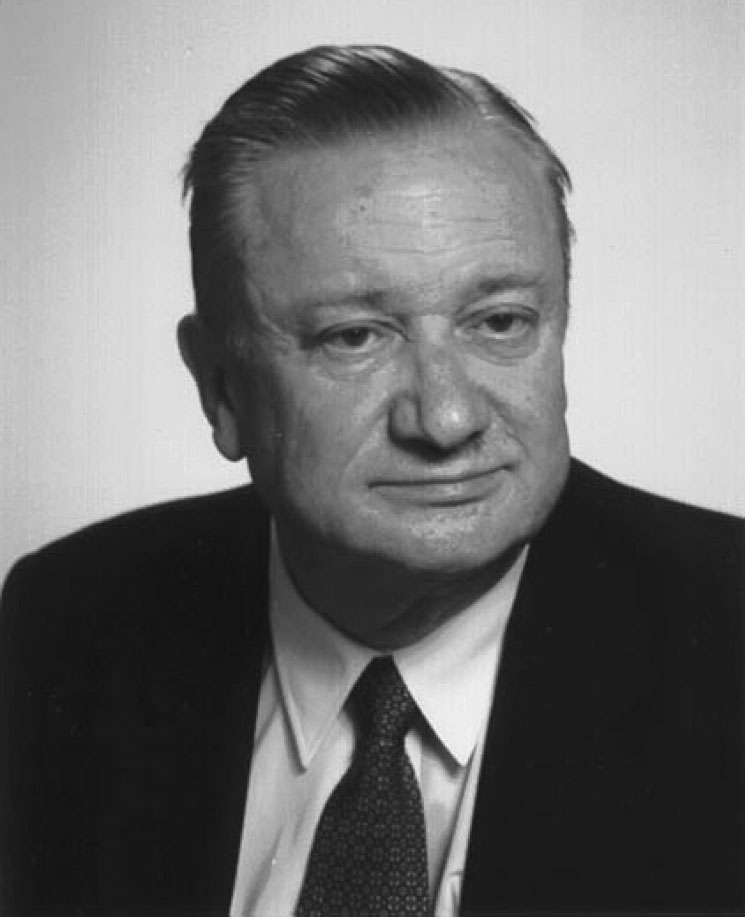
\includegraphics[scale=0.1]{Paul.png}
      \textbf{Paul de Faget de Casteljau \footnotemark[2]}
      %\caption{Pierre Bézier}
    \end{minipage}
  
    \end{figure}}

    \vspace{-2cm}
    \footnotetext[1]{https://macquebec.com/courbes-bezier/}
      \uncover<2->{\footnotetext[2]{http://rocbor.net/Product/surf/PaulDeFagetDeCasteljau.html}}
\end{frame}


\subsection{Applications}
\begin{frame}{Bézier Curves}{Applications}

  \begin{figure}[H]

    \vspace{1cm}
    \hspace{-4cm}
    \begin{minipage}{0.70\linewidth}
      \textbf{Multiple Applications:}
      \begin{itemize}
        \uncover<2->{\item Computer-Aided Design (CAD) }
        \uncover<3->{\item Typeface }
        \uncover<4->{\item Medical Imaging }
        \uncover<5->{\item Easing Functions\\ (cognitive science) }
        \uncover<6->{\item Data Interpolations }
      \end{itemize}
    \end{minipage}

    %\vspace{-2cm}
    \hspace{5cm}
    \begin{minipage}{0.50\linewidth}
      \begin{overprint}
        \onslide<1>
        \vspace{-4cm}
        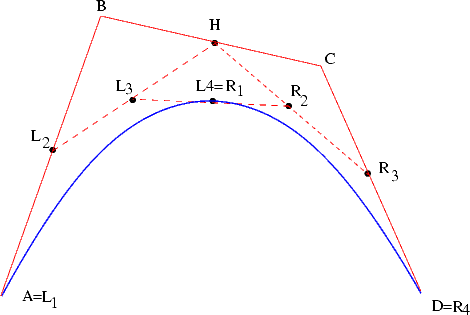
\includegraphics[scale=0.4]{curve.png}
        \begin{center}
        \caption{Quadratic Bézier-Curve\footnotemark[1]}
        \end{center}
        \onslide<2>
        \vspace{-4cm}
        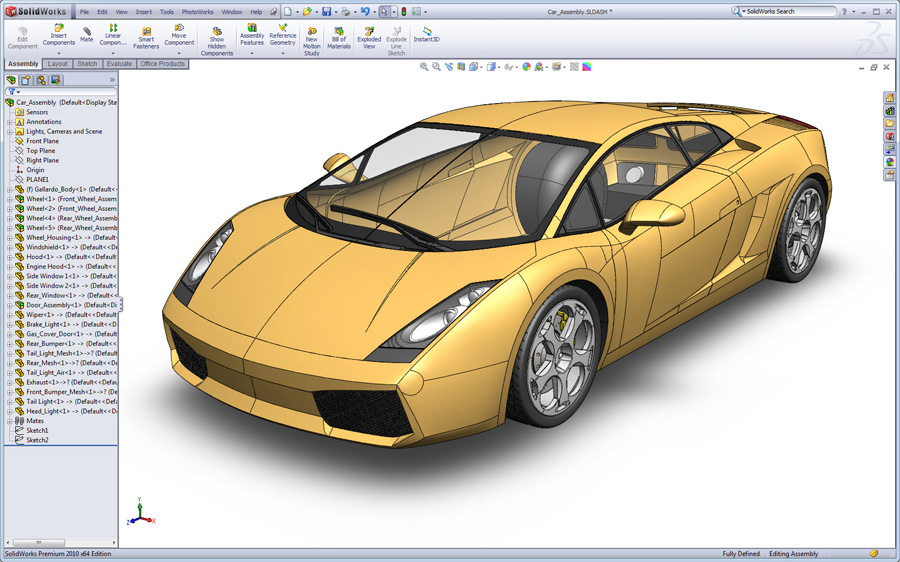
\includegraphics[scale=0.2]{CADcar.png}
        \begin{center}
          \caption{Car model on SolidWorks \footnotemark[2]}
          \end{center}
        \onslide<3>
        \vspace{-3.5cm}
        \begin{center}
          
\includegraphics[scale=0.25]{scripture.png}
          \caption{Exemple of typeface \footnotemark[3]}
        \end{center}
        \onslide<4>
        \vspace{-3.5cm}
        \begin{center}
          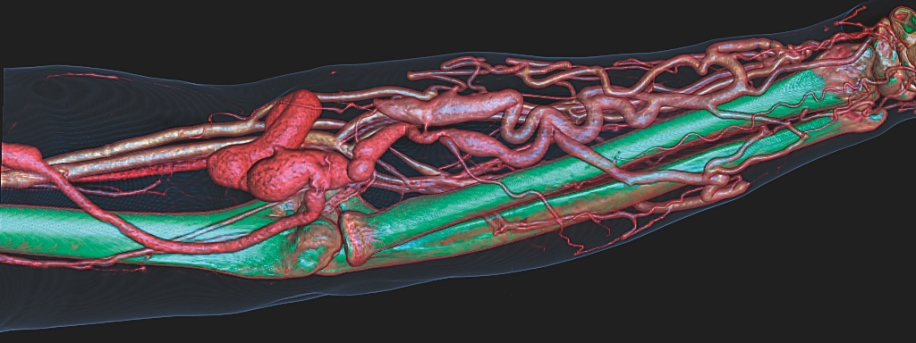
\includegraphics[scale=0.20]{medical.png}
          \caption{Medical Imaging \footnotemark[4]}
        \end{center}
        \onslide<5>
        \vspace{-4cm}
        \begin{center}
           %\hspace{1cm}
          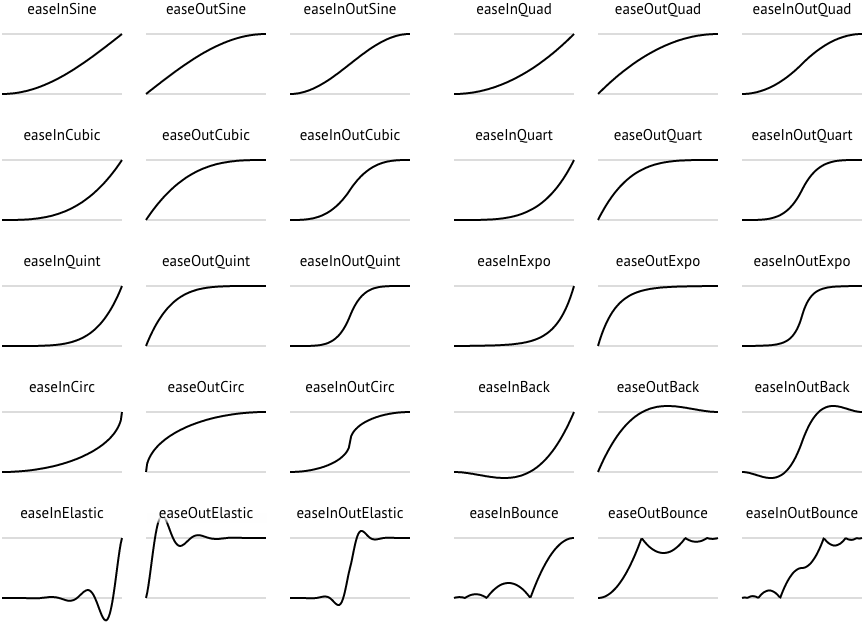
\includegraphics[scale=0.17]{easing.png}
          \caption{Easing Functions \footnotemark[5]}
        \end{center}
        \onslide<6>
        \vspace{-4.5cm}
        \begin{center}
          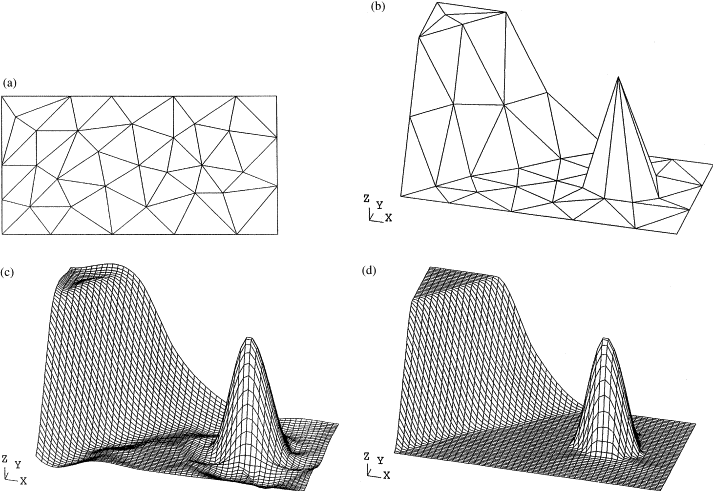
\includegraphics[scale=0.33]{interpolation.png}
          \caption{Data Interpolations \footnotemark[6]}
        \end{center}
    \end{overprint}
    
  \end{minipage}
  
\end{figure}
\vspace{-0.5cm}
\begin{overprint}
  \onslide<1>
  \footnotetext{$^1$https://fr.wikipedia.org/wiki/Courbe\_de\_Bézier}
  \onslide<2>
  \footnotetext{$^2$https://www.quora.com/What-are-the-best-cad-softwares-for-automobile-designing}
  \onslide<3>
  \footnotetext{$^3$https://4design.xyz/courbes-de-bezier-regulieres-illustrator}
  \onslide<4>
  \vspace{-0.25cm}
  \footnotetext{$^4$https://www.siemens.com/innovation/en/home/pictures-of-the-future/health-and-well-being/medical-imaging-dossier.html}
  \onslide<5>
  \footnotetext{$^5$http://easings.net/fr}
  \onslide<6>
  \vspace{-0.25cm}
  \footnotetext{$^6$ Range restricted scattered data interpolation using convex combination of cubic Bézier triangles, E.S.Chan B.H.Ong}
  
\end{overprint}

\end{frame}


\begin{frame}[noframenumbering]{Bézier Curves}{Applications}

  \begin{figure}[H]

    \vspace{1cm}
    \hspace{-4cm}
    \begin{minipage}{0.70\linewidth}
      \textbf{Multiple Applications:}
      \begin{itemize}
      \item Computer-Aided Design (CAD) 
      \item Typeface 
      \item Medical Imaging 
      \item Easing Functions\\ (cognitive science) 
      \item Data Interpolations 
      \item ``Photoshop''... 
      \end{itemize}
    \end{minipage}

    %\vspace{-2cm}
    \hspace{5cm}
    \begin{minipage}{0.50\linewidth}
        \onslide<1>
        \vspace{-4cm}
        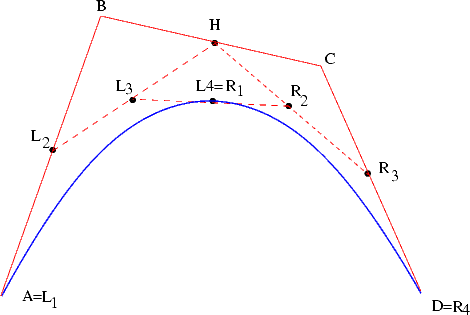
\includegraphics[scale=0.4]{curve.png}
        \begin{center}
        \caption{Wonderfull Photoshop\footnotemark[1]}
        \end{center}
    
  \end{minipage}
  
\end{figure}
\vspace{-0.5cm}
\begin{overprint}

  \footnotetext[1]{Elvira's Photoshop}
 
  
\end{overprint}
\end{frame}

\subsection{Construction}
\begin{frame}{Bézier Curves}{Construction}
  
  \begin{figure}[H]
    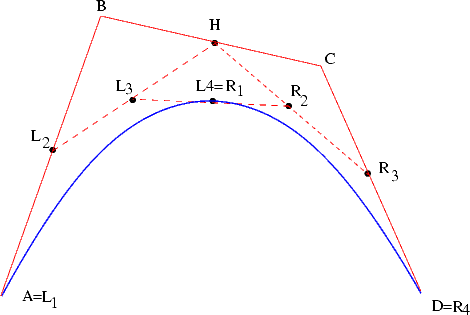
\includegraphics[scale=0.5]{curve.png}
    \caption{Quadratic Bézier Curve}
    (See construction on Geogebra)
  \end{figure}
\end{frame}

  \begin{frame}{Bézier Curves}{Conclusion}

    Why the Bézier Curves are so popular ?
    \begin{itemize}
      \item Intuitive barycentric formulation
      \item Flexible Behaviour
      \item Easy extension to 2D or 3D
      \item Low Memory cost
      \item Various applications
      \item[]
        \uncover<2->{ \item[] ~~~~ and ...}
      \item[]
        \uncover<3->{\item Easily represented in \textbf{Bernstein Polynomial Basis}}
    \end{itemize}
    
  \end{frame}


  \section{Bernstein Polynomials}
  \subsection{Historical Aspect}

\begin{frame}{Bernstein Polynomials}{Historical Aspect}
   \vspace{-0cm}
  \begin{figure}[H]
    \begin{minipage}[top]{0.30\linewidth}
      %\vspace{-2cm}
      \centering
      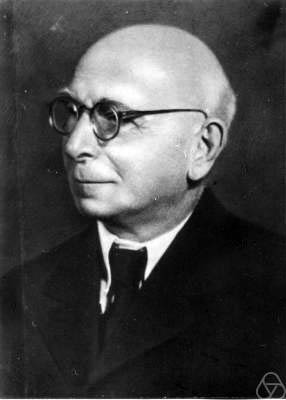
\includegraphics[scale=0.25]{sergei.png}
      \textbf{Sergei Natanowitsch Bernstein \footnotemark[1]}
    \end{minipage}
    \hspace{-2cm}
    \begin{minipage}[top]{0.80\linewidth}


      %\vspace{-2cm}
      \hspace{2cm}
      \textbf{Dates:} \hspace{0.94cm} 1880-1968


      \hspace{2cm}
      \textbf{Nationality:} \hspace{0.09cm} Russian
      
      \hspace{2cm}
      \textbf{Institution:}
      
      \hspace{1cm}
      \vspace{-0.95cm}
      \begin{itemize}
        \item[] \hspace{3.54cm} Sorbonne / Supéléc
        \item[]   \hspace{3.54cm} Kharkov University
          
      \end{itemize}
      \hspace{2cm}
      \textbf{Introduce his polynomial basis in 1912}
      
      
      \begin{center}
        \hspace{2cm}
        $\Rightarrow$ prove the Weierstrass approximation theorem
      \end{center}
      
    \end{minipage}
  \end{figure}

\footnotetext{$^1$ https://fr.wikipedia.org/wiki/Serge\%C3\%AF\_Natanovitch\_Bernstein}
  
\end{frame}

\subsection{Polynomial Forumulation}
\begin{frame}{Bernstein Polynomials}{Polynomial Formulation}

  \begin{figure}[H]
    \hspace{-1.5cm}
    \begin{minipage}[top]{0.40\linewidth}
      Bernstein formulation:
      \begin{flalign*}
        &\begin{aligned}
           B^{N}_{ijkl}=C^{N}_{ijkl}\lambda_0^i\lambda_1^j\lambda_2^k\lambda_3^l \text{~~~ with:~~} C^{N}_{ijkl}=\frac{N!}{i!j!k!l!}
         \end{aligned}&&\\
        &\begin{aligned}
           \text{~~~~~~~~~~~~~~~~~~~~~~~~~~~~~~~~~~~and : ~ }i+j+k+l=N
         \end{aligned}&&
      \end{flalign*}

      \uncover<2->{In 1D it gives :
       \begin{equation}
           B^{N}_{i}(t)=C^{N}_{i}(1-t)^{N-i}t^i
         \end{equation}}
    \end{minipage}
    \begin{minipage}[top]{0.10\linewidth}    
      \definecolor{qqqqff}{rgb}{0,0,1}
      \vspace{0cm}
      \begin{tikzpicture}[scale=0.8]
        %\draw[->,color=black] (-0.24,0) -- (10.1,0);
        %\foreach \x in {,0.5,1,1.5,2,2.5,3,3.5,4,4.5,5,5.5,6,6.5,7,7.5,8,8.5,9,9.5,10}
        %\draw[shift={(\x,0)},color=black] (0pt,2pt) -- (0pt,-2pt) node[below] {\footnotesize $\x$};
        %\draw[->,color=black] (0,-0.67) -- (0,7.71);
        %\foreach \y in {-0.5,0.5,1,1.5,2,2.5,3,3.5,4,4.5,5,5.5,6,6.5,7,7.5}
        %\draw[shift={(0,\y)},color=black] (2pt,0pt) -- (-2pt,0pt) node[left] {\footnotesize $\y$};
        %\draw[color=black] (0pt,-10pt) node[right] {\footnotesize $0$};
        \clip(0.9,0) rectangle (4.3,3.5);
        \draw (1,1)-- (3.08,3.24);
        \draw (4.05,0.47)-- (3.08,3.24);
        \draw (1,1)-- (4.05,0.47);
        \draw [dash pattern=on 1pt off 1pt] (3.09,1.72)-- (1,1);
        \draw [dash pattern=on 1pt off 1pt] (3.09,1.72)-- (3.08,3.24);
        \draw [dash pattern=on 1pt off 1pt] (4.05,0.47)-- (3.09,1.72);
        \begin{scriptsize}
          \fill [color=qqqqff] (1,1) circle (1.5pt);
          \draw[color=qqqqff] (1.07,1.12)  ;
          \fill [color=qqqqff] (4.05,0.47) circle (1.5pt);
          \draw[color=qqqqff] (4.19,0.58) ;
          \fill [color=qqqqff] (3.08,3.24) circle (1.5pt);
          \draw[color=qqqqff] (3.15,3.36)  ;
          \fill [color=qqqqff] (3.09,1.72) circle (1.5pt);
          \draw[color=qqqqff] (3.16,1.84) ;
        \end{scriptsize}
      \end{tikzpicture}\\
      \vspace{-3cm}
       \hspace{-1cm}
     \uncover<2->{\begin{tikzpicture}[scale=3.0]
        \clip(0.09,-0.10) rectangle (1.2,1.04);
        \draw (0.1,0.1)-- (0.5,0.1);
        \draw (0.5,0.1)-- (1.1,0.1);
        \begin{scriptsize}
          \fill [color=qqqqff] (0.1,0.1) circle (0.4pt);
          \draw[color=qqqqff] (0.11,0.11) ;
          \fill [color=qqqqff] (1.1,0.1) circle (0.4pt);
          \draw[color=qqqqff] (1.11,0.11) ;
          \fill [color=qqqqff] (0.5,0.1) circle (0.4pt);
          \draw[color=qqqqff] (0.51,0.11) ;
          \draw[color=black] (0.3,0.05) node {$t$};
          \draw[color=black] (0.81,0.05) node {$1-t$};
        \end{scriptsize}
              \end{tikzpicture}}
      \end{minipage}
  \end{figure}
 \uncover<3>{\textit{NB: Which is equal to the probability of i successes  in trials of N random process with individual probability of t success in each trial.}}
\end{frame}

\subsection{Basis Function Properties}
\begin{frame}{Bernstein Polynomials}{Basis Function Properties}
  
  \begin{figure}[H]
    \hspace{-1.75cm}
    \begin{minipage}[top]{0.60\linewidth}

      Bernstein Basis Properties :
      \begin{itemize}
      \item Highly correlated to probabilities
      \item Partition of unity : $\sum_{k=0}^nB^N_k(t)=1$
      \item Positivity : $\forall t \in [0,1]$, $B^n_k(t)\le0$
      \item Symmetry : $B^N_k(t)=B^N_{N-k}(1-t)$
      \item Describes Bézier curves (See construction on Geogebra)
      \item De Casteljau Algorithm
      \item[]
       \uncover<2->{ \item[] and...
       \item[]}
       \uncover<3->{\item Other interessant proprieties for DGM formulations}
      \end{itemize}     
    \end{minipage}
    \begin{minipage}[top]{0.40\linewidth}
      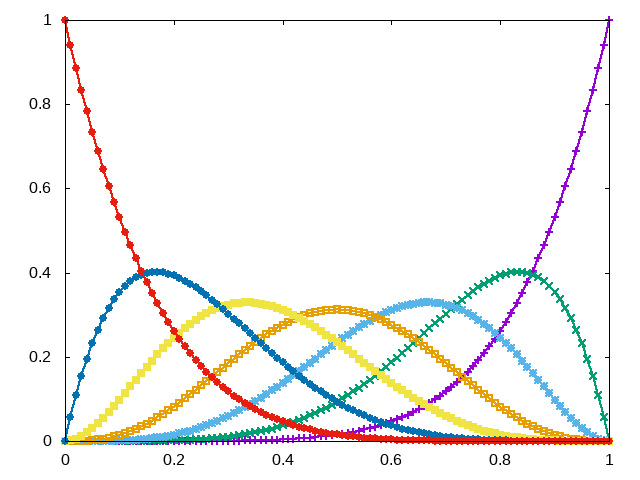
\includegraphics[scale=0.3]{base_b.png}
      \caption{$P[X^6]$ Bersntein basis}
    \end{minipage}
  \end{figure}
\end{frame}

\section{Application on DGs}
\subsection{Useful DGs Properties}
\begin{frame}{Application on DGs}{Useful DGs Properties}


  \begin{figure}[H]
    \begin{minipage}[top]{0.55\linewidth}
      
Bernstein formulation:
      \begin{flalign*}
        &\begin{aligned}
           B^{N}_{ijkl}=C^{N}_{ijkl}\lambda_0^i\lambda_1^j\lambda_2^k\lambda_3^l \text{~~~ with:~~} C^{N}_{ijkl}=\frac{N!}{i!j!k!l!}
         \end{aligned}&&
      \end{flalign*}

       \uncover<2->{Easy Derivative expression:
      \begin{flalign*}
        &\begin{aligned}
           \frac{\partial B_\alpha^N}{\partial \lambda_p}=N B^{N-1}_{\alpha-e_p}  \text{~~~ with:~~} \alpha=(i,j,k,l)
         \end{aligned}&&
      \end{flalign*}}
      
       \uncover<3->{Sparse Degree Elevation operator:
      \begin{flalign*}
        &\begin{aligned}
           B^{N-1}_{\alpha}=\sum_{p=0}^d \frac{\alpha_p+1}{N}B^N_{\alpha+e_p}
         \end{aligned}&&
      \end{flalign*}}
    \end{minipage}\hfill
    \begin{minipage}[bot]{0.36\linewidth}

\vspace{2.5cm}
    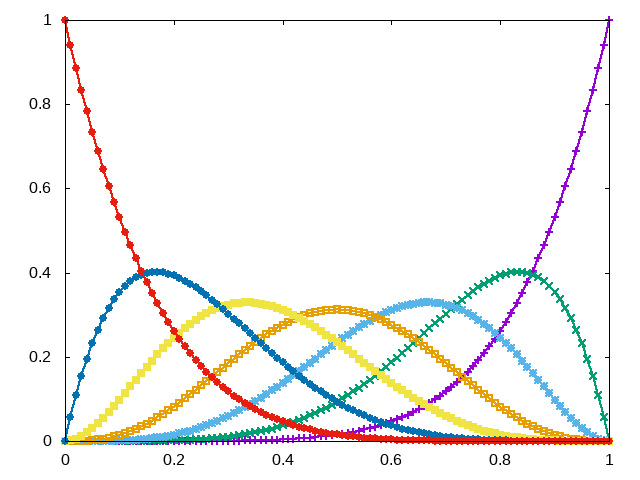
\includegraphics[scale=0.25]{base_b.png}

    ~~~~~~ P[$X^6$] Bernstein basis

 %% \uncover<5->{\vspace{2.5cm}
 %%  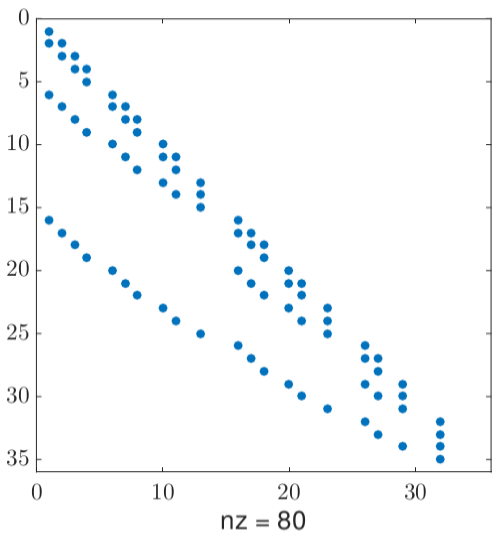
\includegraphics[scale=0.25]{sparse.png}

 %% ~~~~~ P[$X^6$] Bernstein basis}
     \end{minipage}\hfill
    \end{figure}
    
  \end{frame}



\begin{frame}{Application on DGs}{Useful DGs Properties}

  Unique boundary condition values :

  \begin{figure}[H]
    \subfigure[P($X^6$) Lagrange basis]{
      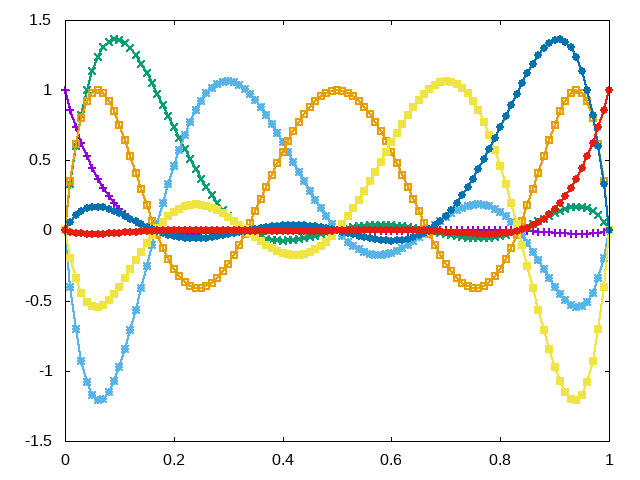
\includegraphics[scale=0.30]{base_l.png}
    }
    \subfigure[P($X^6$) Bernstein basis]{
      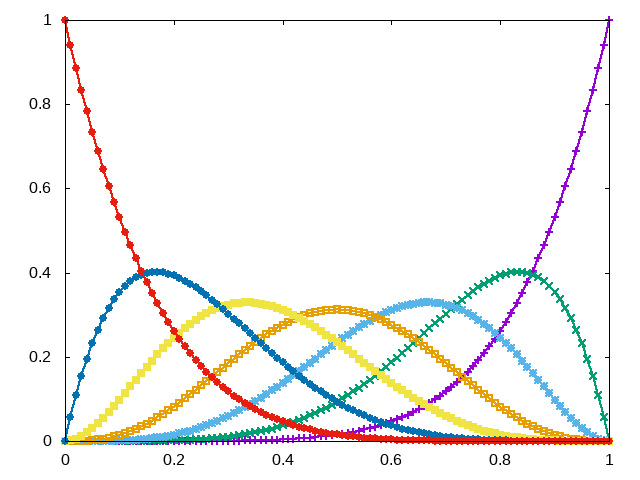
\includegraphics[scale=0.30]{base_b.png}
    }
  \end{figure}
  
  $\Rightarrow$ Same Flux Management
\end{frame}

\subsection{Discontinuous Galerkin formulation}
\begin{frame}{Application on DGs}{Discontinuous Galerkin formulation}
  First order Acoustic Wave equation discretisation: 
  \begin{multicols}{2}
    Continuous Problem: \\
    \begin{empheq}[left=\empheqlbrace]{align}
      & \frac{\partial p}{\partial_t}+\kappa_0 div(\overrightarrow u)=0      \label{ac1_2}  \\
      & \rho_0 \frac{\partial \overrightarrow u}{\partial_t}+ \overrightarrow{grad}(p)=0  \label{ac1_1} 
    \end{empheq}
    
    
    \columnbreak
    Discrete Problem:
    \vspace{0.25cm}
    \begin{empheq}[left=\empheqlbrace]{align}
      & M \frac{\partial P}{\partial_t}+\sum_d S_dU_d=M^FF_p \\
      & M \frac{\partial U_d}{\partial_t}+S_dP=M^FF_{u}
    \end{empheq}
  \end{multicols}

  \uncover<2->{
  With $Sd=MD_d$  and $Lift=M^{-1}M^F$:

      \begin{empheq}[left=\empheqlbrace]{align}
      &  \frac{\partial P}{\partial_t}+\sum_d D_dU_d=Lift F_p \\
      &  \frac{\partial U_d}{\partial_t}+D_dP=Lift F_{u}
    \end{empheq}}
  
\end{frame}

\subsection{Operator Evaluation}
\begin{frame}{Application on DGs}{Operator Evaluation}

  \begin{figure}

    \subfigure[3D Lagrange D matrix]{
      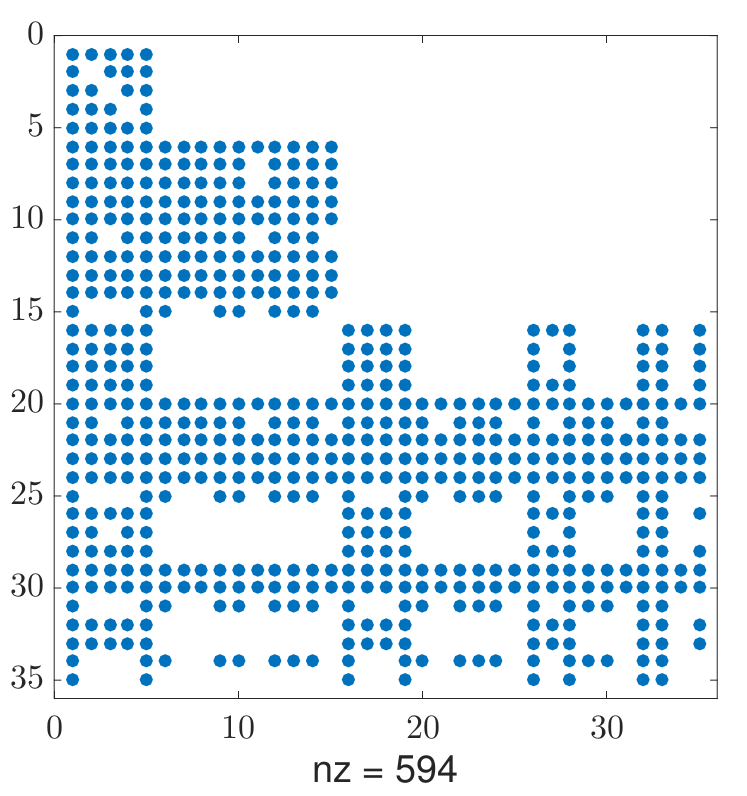
\includegraphics[scale=0.17]{nodalD.png}
    }
    \hspace{1.5cm}
    \subfigure[3D Bernstein D matrix]{
      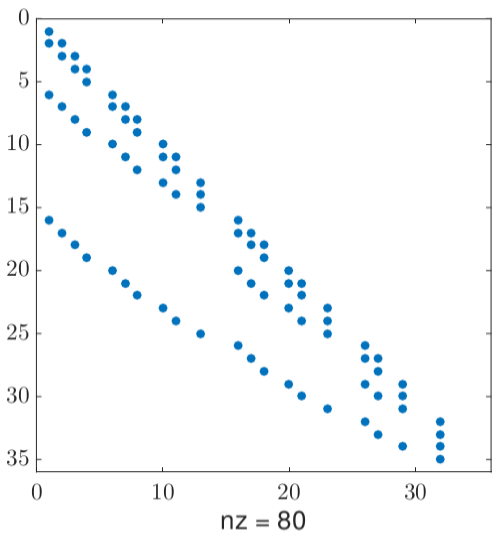
\includegraphics[scale=0.24]{sparse.png}
    }
  \end{figure}

  %% pour mettre en bas et en petit
  \vfill
  \tiny
  %%%%%%%%%%%%%%%%%%%%%%%%%%%%%%%%%%
  \begin{thebibliography}{1}
  \bibitem{chan2017gpu} Chan Jesse and Warburton T. 
    \newblock GPU-Accelerated Bernstein Bézier Discontinuous Galerkin Methods for Wave Problems
    \newblock SIAM Journal on Scientific Computing 2017
  \end{thebibliography}
\end{frame}


\begin{frame}{Application on DGs}{Operator Evaluation}

  \vspace{-0.5cm}
  \begin{figure}
    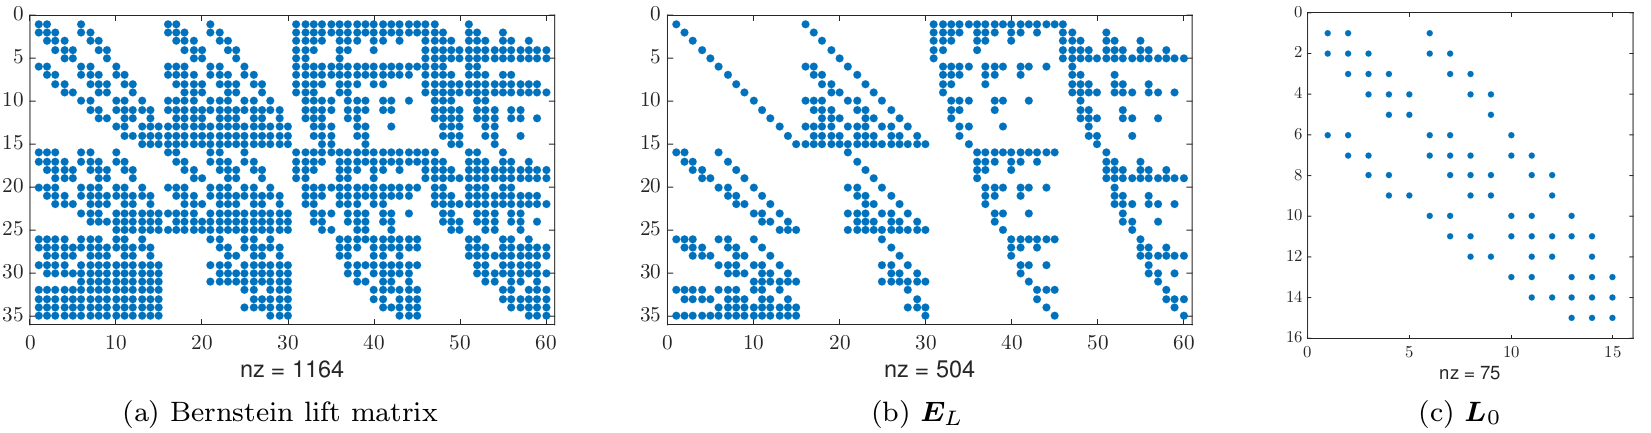
\includegraphics[scale=0.27]{liftmatrix.png}
    Bernstein Lift matrix operator decomposition
  \end{figure}
  \vspace{0.5cm}
  With $Lift=E_L*L_0$

  %% pour mettre en bas et en petit
  \vfill
  \tiny
  %%%%%%%%%%%%%%%%%%%%%%%%%%%%%%%%%%
  \begin{thebibliography}{3}
  \bibitem{chan2017gpu} Chan Jesse and Warburton T. 
    \newblock GPU-Accelerated Bernstein Bézier Discontinuous Galerkin Methods for Wave Problems
    \newblock SIAM Journal on Scientific Computing 2017
  \end{thebibliography}
\end{frame}

\begin{frame}{Application on DGs}{Few Personal Results}

    \begin{figure}[H]
      \begin{minipage}{0.7\linewidth}
        \begin{empheq}[left=\empheqlbrace]{align}
          & P^{n+\frac{1}{2}}=P^{n-\frac{1}{2}}+A_pU^{n}+RHS_p     \\
          & U^{n+1}=U^{n}+A_uP^{n+\frac{1}{2}}+RHS_u   
        \end{empheq}
      \end{minipage}

      \vspace{0.5cm}
      \begin{minipage}{0.70\linewidth}
        \centering
        \movie[showcontrols=true,width=4.9cm,height=4cm]
              {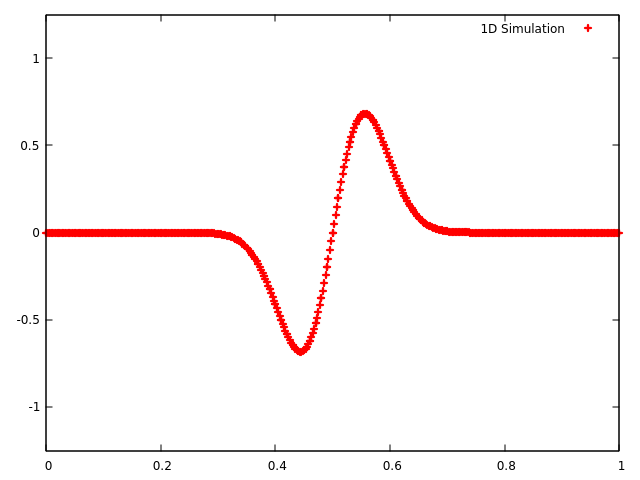
\includegraphics[width=4.9cm,height=4cm]
                {anime1.png}}
              {animate.mp4}
              \caption{First 1D DG Simulation}
      \end{minipage}
    \end{figure}
  \end{frame}


\begin{frame}{Application on DGs}{Few Personal Results}    
    \begin{figure}[H]
      \begin{minipage}[top]{0.50\linewidth}
        \centering
        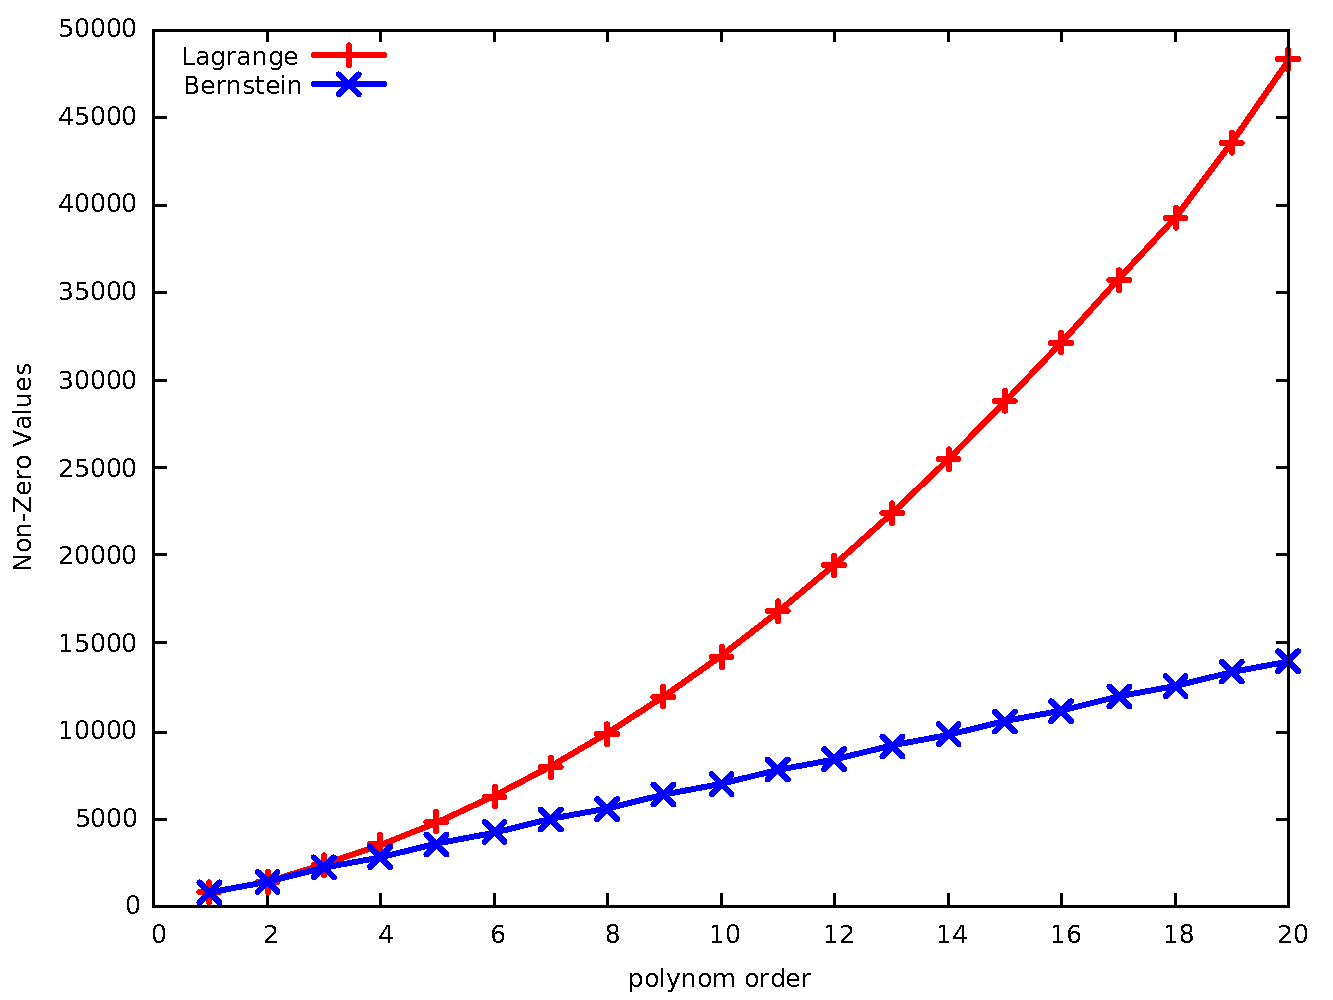
\includegraphics[scale=0.24]{bernstein1.pdf}
        \footnotesize
        %\begin{center}
        $A_p/A_u$ NZVs as a function of the order
        %  \end{center}
        \normalsize
      \end{minipage}
      \hspace{-0.3cm}
      \begin{minipage}[top]{0.50\linewidth}
        \centering
        %\vspace{-0.3cm}
        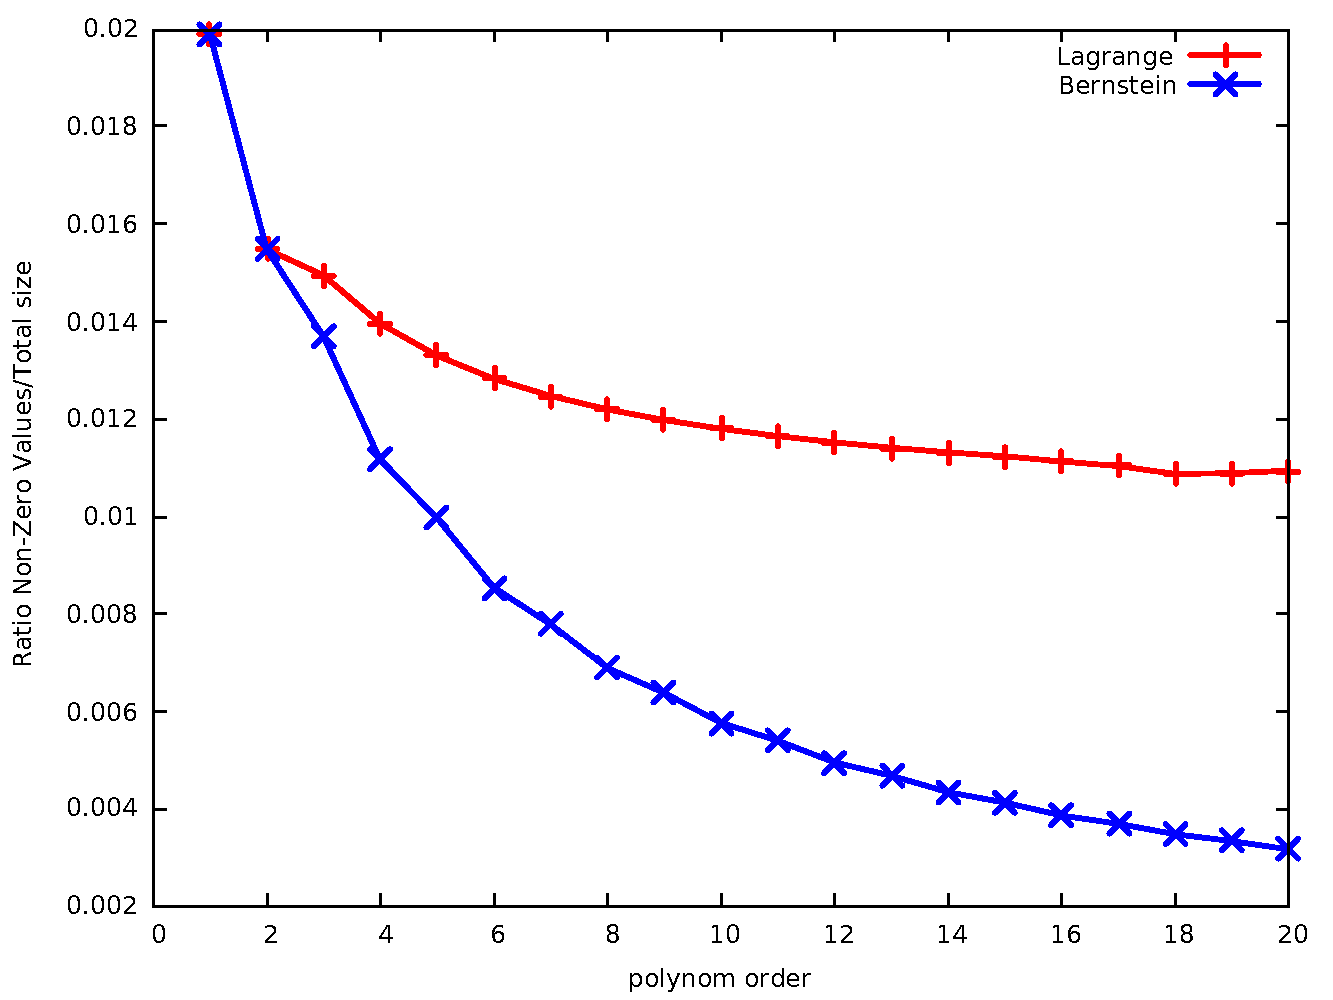
\includegraphics[scale=0.24]{bernstein2.pdf}
        \footnotesize
        % \begin{center}
        $A_p/A_u$ NZVs Ratio $(NZVs/Size)$
        \normalsize
        %  \end{center}
      \end{minipage}\hfill
    \end{figure}
\end{frame}

\subsection{Conclusion}
\begin{frame}{Application on DGs}{Conclusion}

  Main results about Bernstein-Bézier polynomial basis :
  \begin{itemize}
  \item Plenty of utilization of Bézier curves
  \item Plenty of numerical properties of Bernstein polynomial basis
  \item Recently used in numerical simulation
  \item Create very Sparse Matrices
  \item Same Flux management as a nodal polynomial basis
  \item Easy elevation/reduction degree (useful for p-adaptivity)
  \item Easy Derivative
  \end{itemize}


\end{frame}

%% \begin{frame}{Bibliography}
%% \bibliographystyle{unsrt}
%% \bibliography{bibliographie}
%% \end{frame}

\end{document}
